\section{Vergleich von TCP Reno und TCP Cubic}

\textit{Hinweis zur Gliederung: Die Darstellung folgt dem Ablauf des Experiments und weicht deshalb von der Reihenfolge der Teilaufgaben a bis d ab. Die Teilaufgaben 3a und 3b werden in Abschnitt~\ref{sec:reno-cubic-parameter} behandelt. Die Analyse aus Teilaufgabe 3c wird in Abschnitt~\ref{sec:reno-cubic-methodik} beschrieben. Vergleich und Bewertung gemäß Teilaufgabe 3d erfolgen in den Abschnitten~\ref{sec:reno-cubic-ergebnisse} und~\ref{sec:reno-cubic-diskussion}.}

\subsection{Parameter und Durchführung}\label{sec:reno-cubic-parameter}

\subsubsection{Setup}

Beide Experimente nutzen das gleiche Netzwerk (vgl.\ Abschnitt~\ref{sec:aufbau}) mit identischen Linkparametern.
Die Konfigurationen sind in \texttt{lab-reno.yaml} und \texttt{lab-cubic.yaml} definiert.
Die gemeinsamen Linkparameter sind in Tabelle~\ref{tab:reno_cubic_link} zusammengefasst.

\begin{table}[h]
    \centering
    \begin{tabular}{|l|r|}
        \hline
        \textbf{Parameter} & \textbf{Wert} \\ \hline
        Bandbreite & 1\,Mbit/s \\ \hline
        Verzögerung (One-Way) & 20\,ms \\ \hline
        Jitter & 0\,ms \\ \hline
        Paketverlustrate & 3\,\% \\ \hline
        Burst & 32\,kbit \\ \hline
    \end{tabular}
    \caption{Linkparameter für beide Experimente}\label{tab:reno_cubic_link}
\end{table}

Zur Messung wird iperf3 (vgl.\ Abschnitt~\ref{sec:iperf3_docker_tool}) verwendet.
Der Sender (n1), als iperf3-Client, sendet über 30\,Sekunden Daten an den Empfänger (n2), der als iperf3-Server agiert.
Die Ergebnisse werden im JSON Format auf Sekundenbasis als Messerintervalle gespeichert.
Zudem werden PCAP Dateien auf beiden Seiten generiert.

\subsubsection{Durchführung mit TCP Reno}

Für den ersten Durchlauf wird TCP Reno als Staukontrolle konfiguriert (vgl.\ \texttt{lab-reno.yaml}).
Anschließend wird Messung mittels iperf3 gestartet und Traffic aufgezeichnet.

\subsubsection{Durchführung mit TCP Cubic}

Im zweiten Experiment wird die Staukontrolle auf TCP CUBIC gewechselt (vgl.\ \texttt{lab-cubic.yaml}).
Die restlichen Einstellungen bleiben unverändert.
Zuletzt wird unter gleichen Bedingungen die Messung durchgeführt.

\subsubsection{Messdaten}

Aus jedem Experiment ergeben sich drei Dateien:
\begin{itemize}
    \item \texttt{iperf3\_\{reno,cubic\}.json} : Durchsatz, Retransmissionen und cwnd
    \item \texttt{tcp\_\{reno,cubic\}.pcap} : PCAP auf Senderseite
    \item \texttt{tcp\_\{reno,cubic\}\_receiver.pcap} : PCAP auf Empfängerseite
\end{itemize}

\FloatBarrier{}
\subsection{Ergänzende Methodik}\label{sec:reno-cubic-methodik}

\subsubsection{Durchsatzanalyse}

Der Durchsatz kann direkt aus den iperf3 Dateien entnommen werden.
Für jedes der Messintervalle wird Bitrate und Zeitstempel extrahiert.

\subsubsection{Analyse des Staukontrollfensters}

Zur Analyse der Staukontrollfenster wird \texttt{tcptrace}~\cite{tcptrace} auf die Sender PCAPs angewendet.
Das Tool erzeugt \texttt{xpl}-Dateien mit dem Outstanding-Data-Verlauf, also der Menge an gesendeten, aber noch nicht bestätigten Daten.
Laut Man-Page approximiert dieser Wert das Congestion Window (\textit{estimated congestion window})~\cite{tcptrace}.
Aus der durch tcptrace erzeugten Datei werden die Daten der Kategorie \texttt{red} entnommen, die den Outstanding Wert gegenüber der Zeit darstellen.

\subsubsection{Retransmissionen und Paketverluste}

Retransmissionen werden mit \texttt{tshark} aus den Sender PCAPs extrahiert.
Dabei wird durch \texttt{tcp.analysis.retransmission} alle Pakete gefiltert, die von TCP als Retransmission erkannt werden.
Für jedes dieser Pakete wird der relative Zeitstempel gespeichert.

Zur Bestimmung der Paketverluste werden Sender und Empfänger PCAPs verglichen.
Aus beiden Aufzeichnungen werden alle Pakete mit (\texttt{tcp.len > 0}) und (\texttt{ip.id}) extrahiert.
Anschließend wird in Python die Mengendifferenz berechnet: $\text{Lost} = \{ x \in \text{Sender} \mid x \notin \text{Receiver} \}$.

\subsubsection{Auswertungsskripte}

Die gesamte Analyse ist über den Orchestrator \texttt{analyze.sh} idempotent ausführbar.
Dieses ruft nacheinander \texttt{tcptrace-util.sh} (in einem \texttt{debian:bookworm-slim} Docker Container), \texttt{tshark-util.sh} und \texttt{analyze.py} (via \texttt{uv run}) auf.
Das Python Skript nutzt \texttt{parsers.py} für das Parsing der Dateien sowie \texttt{plots.py} für die Erzeugung der Diagramme mit \texttt{matplotlib}.
Voraussetzungen für die Ausführung sind \texttt{docker}, \texttt{tshark} und \texttt{uv}.

\FloatBarrier{}
\subsection{Ergebnisse}\label{sec:reno-cubic-ergebnisse}

\subsubsection{Durchsatz}

Abbildung~\ref{fig:throughput_comparison} zeigt den Durchsatzverlauf beider Algorithmen über die eingestellte Dauer.

\begin{figure}[h!]
    \centering
    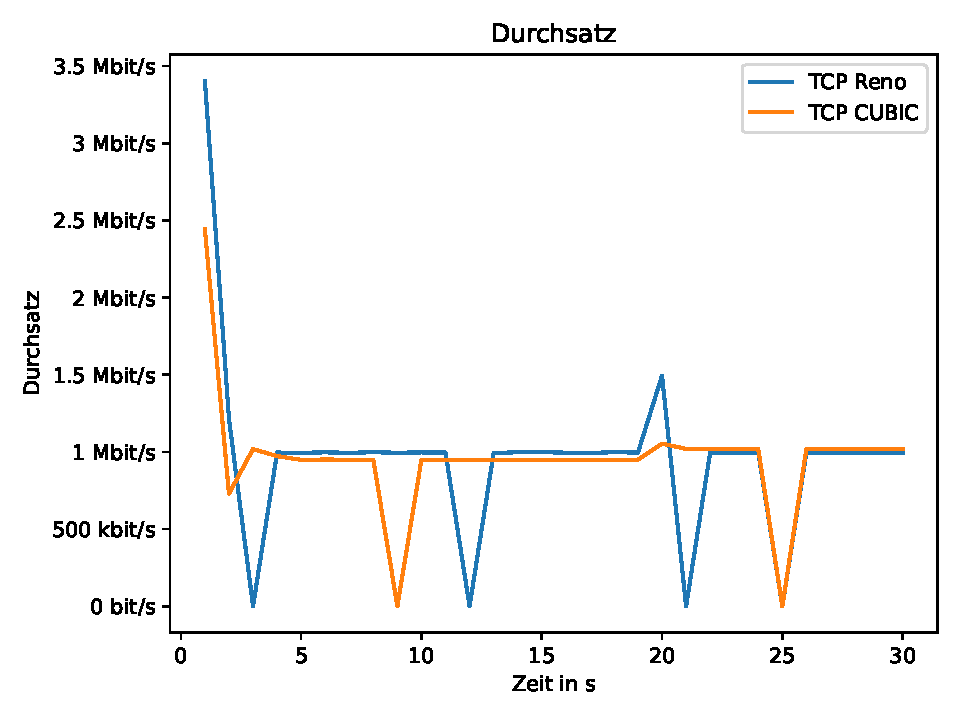
\includegraphics[width=0.9\textwidth]{res/03-reno-cubic/analysis/throughput-comparison.pdf}
    \caption{Durchsatzverlauf von TCP Reno und TCP CUBIC}\label{fig:throughput_comparison}
\end{figure}

Der mittlere Durchsatz wird von iperf3 als \texttt{bits\_per\_second} unter \texttt{end.sum\_sent} in \texttt{iperf3\_\{reno,cubic\}.json} dargestellt.
TCP Reno misst ca.\ 968\,kbit/s, TCP CUBIC ca.\ 956\,kbit/s.
Die Werte liegen damit nahe an der Konfiguration von 1\,Mbit/s Durchsatz.
Beide Algorithmen zeigen Schwankungen, welche auf die konfigurierte Paketverlustrate von 3\,\% zurückzuführen sind.
Aus \texttt{end.sum\_sent} ergeben sich \texttt{bytes} und \texttt{retransmits}: Reno überträgt 3.628.688\,Bytes mit 80 Retransmissionen, CUBIC 3.586.696\,Bytes mit 71 Retransmissionen.

\FloatBarrier{}
\subsubsection{Entwicklung des Staukontrollfensters}

Abbildung~\ref{fig:cwnd_comparison} zeigt den Verlauf der Outstanding Data (approx.\ Congestion Window) beider Algorithmen im Vergleich.

\begin{figure}[h!]
    \centering
    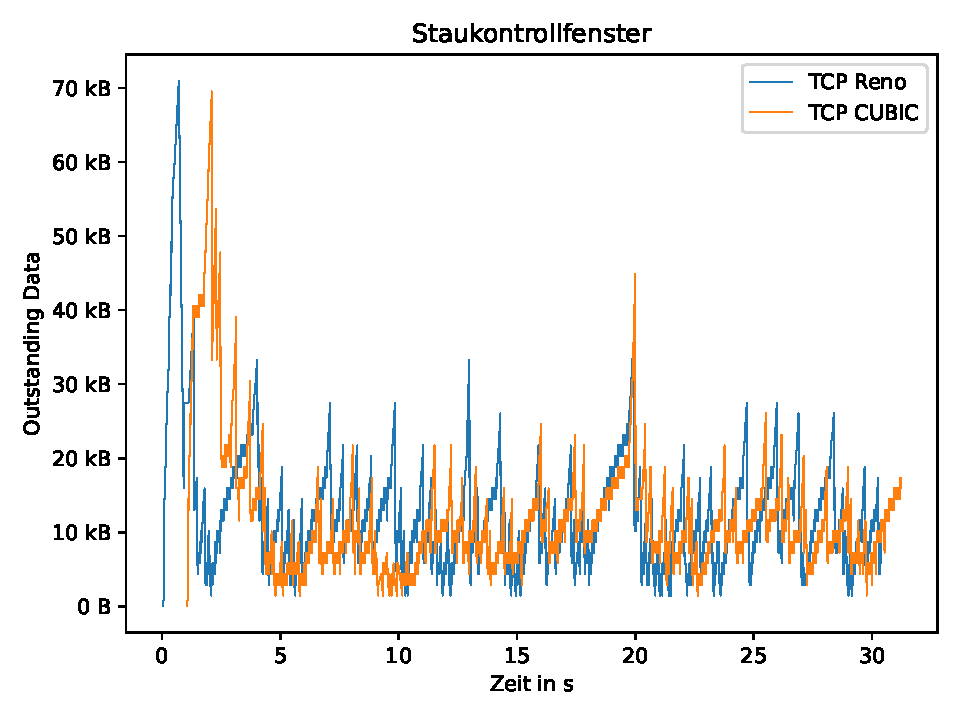
\includegraphics[width=0.9\textwidth]{res/03-reno-cubic/analysis/cwnd-comparison.pdf}
    \caption{cwnd von TCP Reno und TCP CUBIC}\label{fig:cwnd_comparison}
\end{figure}

Bei TCP Reno zeigt sich das typische Muster: cwnd wächst linear in der Congestion Avoidance, bis ein Paketverlust erkannt wird, woraufhin es halbiert wird.
Aus der tcptrace Zusammenfassung (\texttt{reno-summary.txt}) ergeben sich \texttt{max owin} = 70.953\,Bytes und \texttt{avg owin} = 12.232\,Bytes.
Zum Vergleich zeigt iperf3 \texttt{snd\_cwnd} im Bereich von 2.896 bis 27.512\,Bytes (Mittel: 10.667\,Bytes).
Abbildung~\ref{fig:cwnd_losses_reno} zeigt den Zusammenhang mit den Paketverlusten: 82 verlorene Pakete (Verlustrate 3,4\,\%).

\begin{figure}[h!]
    \centering
    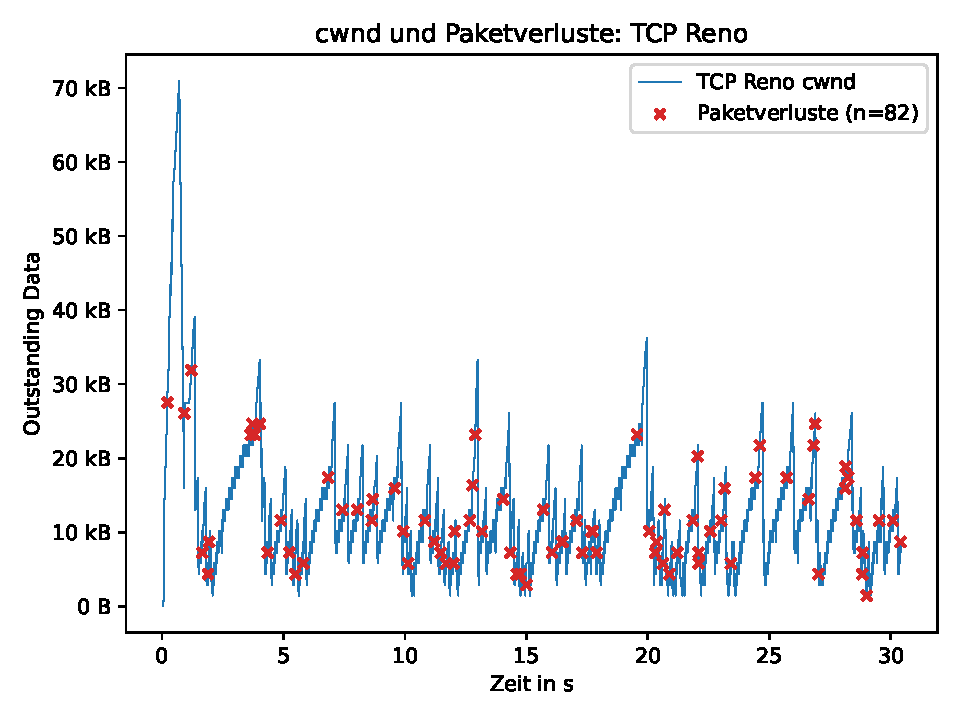
\includegraphics[width=0.9\textwidth]{res/03-reno-cubic/analysis/cwnd-losses-reno.pdf}
    \caption{cwnd und Paketverluste von TCP Reno}\label{fig:cwnd_losses_reno}
\end{figure}

\FloatBarrier{}

TCP CUBIC zeigt ein aggressiveres Wachstumsverhalten.
Im Verlauf zeigt sich nach jedem Verlustereignis ein Abfall des cwnd auf etwa 70\,\% des zuvor erreichten Maximums. Der Anstieg verläuft zunächst steil, flacht beim Erreichen des vorherigen Maximalwerts sichtbar ab und geht dort in ein Plateau über.
Laut \texttt{cubic-summary.txt}: \texttt{max owin} = 69.505\,Bytes, \texttt{avg owin} = 11.980\,Bytes.
Vergleichsweise zeigt iperf3 \texttt{snd\_cwnd} von 1.448 bis 28.960\,Bytes (Mittel: 10.570\,Bytes).
Abbildung~\ref{fig:cwnd_losses_cubic} zeigt die Paketverluste: TCP CUBIC weist 70 verlorene Pakete auf (Verlustrate 2,9\,\%).

\begin{figure}[h!]
    \centering
    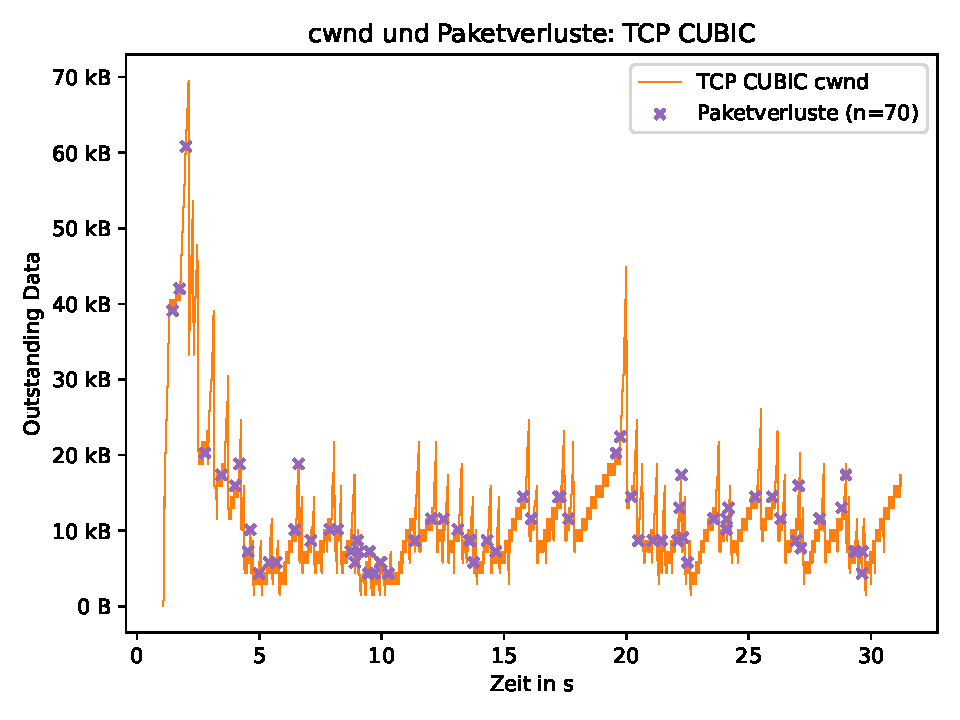
\includegraphics[width=0.9\textwidth]{res/03-reno-cubic/analysis/cwnd-losses-cubic.pdf}
    \caption{cwnd und Paketverluste von TCP CUBIC}\label{fig:cwnd_losses_cubic}
\end{figure}

\FloatBarrier{}
\subsubsection{Retransmissionen, Paketverluste und deren Einfluss}

Abbildung~\ref{fig:retransmission_comparison} stellt die kumulierten Retransmissionen beider Algorithmen als Stufenfunktion dar.

\begin{figure}[h!]
    \centering
    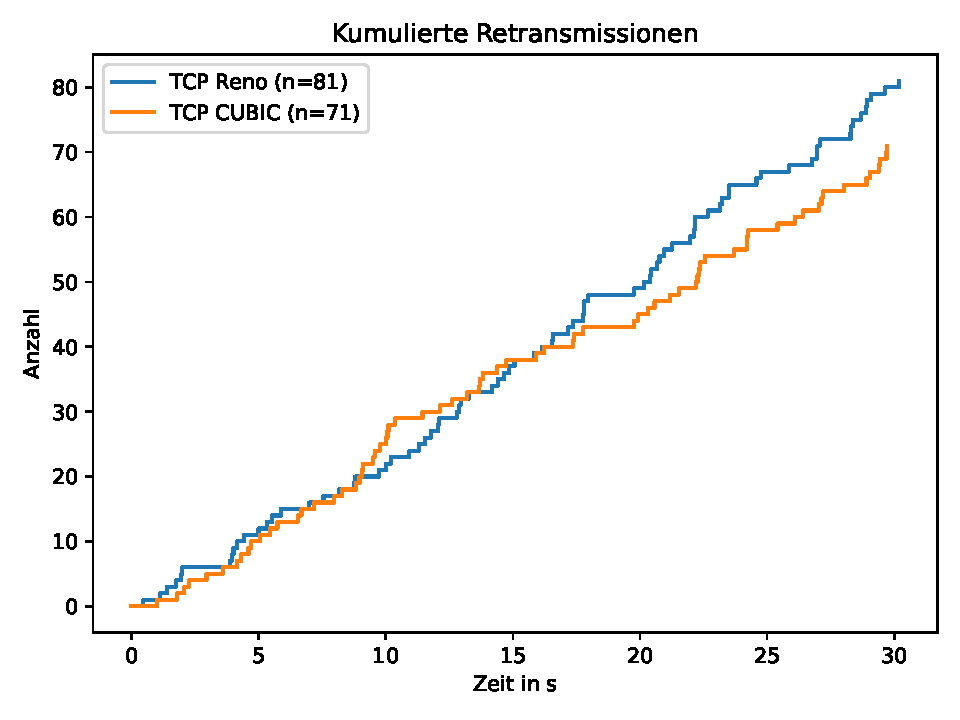
\includegraphics[width=0.9\textwidth]{res/03-reno-cubic/analysis/retransmissions-comparison.pdf}
    \caption{Kumulierte Retransmissionen von TCP Reno und TCP CUBIC}\label{fig:retransmission_comparison}
\end{figure}

TCP Reno zeigt insgesamt 81 Retransmissionen, TCP CUBIC 71.
Die Retransmissionsrate steigt bei beiden Algorithmen annähernd gleichmäßig an, was mit der Paketverlustrate von 3\,\% konsistent ist.

Der Zusammenhang zwischen Paketverlusten und Staukontrollfenster ist wie bereits beschrieben in Abbildung~\ref{fig:cwnd_losses_reno} und Abbildung~\ref{fig:cwnd_losses_cubic} sichtbar.
"Hier gleich den näheren mathematischen vergleich von differentielle Verlaufsanalyse oder, näher an der Statistik, regressionsbasierte Modellselektion. UND ereignisbasierte Latenzanalyse oder formaler Punktprozessanalyse der Paketverluste mit Regime änderung"
\FloatBarrier{}
\subsubsection{Zusammenfassender Vergleich}

Tabelle~\ref{tab:reno_cubic_summary} fasst die wichtigsten Kennwerte beider Algorithmen zusammen (Entnommen aus \texttt{iperf3\_\{reno,cubic\}.json}, \texttt{\{reno,cubic\}-summary.txt} und \texttt{parse\_packet\_losses()} in \texttt{parsers.py}).

\begin{table}[h]
    \centering
    \begin{tabular}{|l|r|r|}
        \hline
        \textbf{Kennzahl} & \textbf{TCP Reno} & \textbf{TCP CUBIC} \\ \hline
        Mittlerer Durchsatz & 968\,kbit/s & 956\,kbit/s \\ \hline
        Übertragene Bytes & 3.628.688 & 3.586.696 \\ \hline
        Retransmissionen & 81 & 71 \\ \hline
        Paketverluste & 82 & 70 \\ \hline
        Verlustrate & 3,4\,\% & 2,9\,\% \\ \hline
        Max.\ Outstanding Data & $\approx$\,71\,kB & $\approx$\,70\,kB \\ \hline
        Mittl.\ Outstanding Data & $\approx$\,12\,kB & $\approx$\,12\,kB \\ \hline
        RTT (Mittel) & 91,4\,ms & 86,2\,ms \\ \hline
        RTT (Min / Max) & 40,3 / 437,2\,ms & 40,1 / 340,1\,ms \\ \hline
        Triple Dupacks & 59 & 52 \\ \hline
    \end{tabular}
    \caption{Vergleich der Kennwerte}\label{tab:reno_cubic_summary}
\end{table}

\FloatBarrier{}
\subsection{Diskussion}\label{sec:reno-cubic-diskussion}

\subsubsection{Wachstum und Reaktion}

\subsubsection{Performance, Robustheit und Stabilität}

\subsubsection{Praktischer Einsatz}

\subsubsection{Grenzen des Labs}

Das Experiment unterliegt einigen Einschränkungen, die bei der Interpretation berücksichtigt werden müssen:

\begin{itemize}
        \item Die künstlich erzeugte Paketverlustrate von 3\,\% liegt über realistischen Werten.
        \item Die Bandbreite von 1\,Mbit/s führt zu einem niedrigen BDP.
        \item Die kurze Messdauer von 30\,Sekunden begrenzt die Aussagekraft.
        \item Die Linux-Implementierungen können vom RFC abweichen.
        \item Das Einstellen der Algorithmen könnte im Experiment unvollständig gewesen sein.
\end{itemize}
